\section{Development After Independent Review}\label{sec:revision}
The original frozen protocols and their outcomes are unchanged. This section
reports subsequent development, including negative experimental sensitivity
results. It does not establish that the current method meets the usefulness
requirements raised by the independent review.
The old frozen evaluators abort on detected undercoverage before retaining the
offending record. Neither completed study encountered that branch, but the
failure policy was flawed. Their source remains reproducible; new diagnostic
evaluators persist results before flagging an audit failure.

\subsection{Matrix-free shared fields and a numerical failure budget}
Each first or second pose-derivative field is a Fourier sum multiplied by one of
ten monomials $1,x,y,z,x^2,y^2,z^2,xy,xz,yz$. Summing coefficient combinations
before transforming gives a field/adjoint pair with ten type-3 NUFFTs per
direction. No global particle-by-particle field Gram is formed. Positive group
scales $d_j$ may come from streamed block norms or from polynomial coefficient
envelopes. They need not equal exact block norms. Identically zero blocks may
be omitted; blocks that can become nonzero during optimization require positive
scales. Particle-specific pose radii are accepted.

An approximate leading eigenvalue is insufficient for an upper audit. Random
starts have a long history in spectral estimation \citep{kw1992}; the following
elementary construction states our particular numerical probability budget.
For a fixed positive semidefinite $C=FF^\top$, draw $m$ independent standard
Gaussian probes $g_j$, independently of the estimator-selection process. Set
$c=\sqrt{2}\,\operatorname{erf}^{-1}(\delta^{1/m})$. Fix a leading unit
eigenvector $v$ before the draws. Since
\[
 \Pr\{\max_j|v^\top g_j|<c\}=\delta,
\]
with probability at least $1-\delta$, simultaneously for every integer $p\ge1$,
\begin{equation}
 \lambda_{\max}(C)
 \le \left(\frac{\max_j\norm{C^p g_j}}{c}\right)^{1/p}.
 \label{eq:randompower}
\end{equation}
The proof retains the leading eigenvector component of $C^p g_j$ in its norm.
Stable normalization tracks the product of norms in log space. The minimum
across powers is valid on the same event; a deterministic trace bound may cap
it. A Rayleigh value is recorded only as a lower diagnostic.

Add the analytic integration pad to this spectral upper value before using the
shared-field inequality. Allocate $\alpha_{\rm noise}+\delta\le\alpha$. A union
bound then includes numerical randomization in the stated failure budget.
Candidate selection using the same probes is not licensed: weights and scales
must be fixed before fresh final probes, or all candidates need a simultaneous
budget. Operator roundoff and NUFFT approximation remain numerical checks,
not validated arithmetic.

Completed radius-five audits with 128 and 1,024 particles take 50.3 and 353.3
seconds under concurrent Mac load, with measured peak resident memory of 390
and 434 MB. Their relative half-widths are 0.438 and 0.740, respectively. They
use different fitted estimators, so the latter result does not measure a
particle-count benefit. The 128-particle randomized field bound is 1.157 times
the dense comparator. A distinct 10,000-particle, radius-12 audit is in progress;
no completed scale or usefulness result is inferred from launching it.

\subsection{Including pose uncertainty in estimator optimization}
Fix the group scales, let $F(w)$ be the scaled quadrature field matrix, and let
$a_q(w)$ be each real/imaginary weight pair's Euclidean amplitude. A nonnegative
matrix $M$ maps these amplitudes to polynomial coefficient envelopes. With
integration constant $E$, $R=B+P$, and integrated cubic coefficients $r_q\ge0$,
the revised sum objective is
\begin{align}
 J(w)&=z\norm{w}+B\norm{\ell-\A^*w}+p(w)
       +\sum_q r_q a_q(w),\nonumber\\
 p(w)&=R\sqrt{\sum_jd_j}
 \sqrt{\norm{F(w)}_{\rm op}^2+E\norm{Ma(w)}^2}.
 \label{eq:poseoptimized}
\end{align}
This is convex: $F$ is linear, $M$ is nonnegative, and the Euclidean norm is
monotone on the nonnegative orthant. It is an upper objective for the prescribed
class, not the exact minimax nonlinear-pose risk. Approximate singular modes
and log-sum-exp smoothing guide numerical optimization. The final primal upper
audit uses Equation~\eqref{eq:randompower} with fresh probes.

A feasible dual lower bound remains available without an optimizer-success
claim. Choose $v\in H$ and supporting linear functionals $g_p,g_r$ such that
\begin{align*}
 \norm{v}&\le B,&\norm{\A v-g_p-g_r}&\le z,\\
 g_p^\top x&\le p(x),&
 g_r^\top x&\le\sum_qr_q a_q(x)\quad\text{for all }x.
\end{align*}
The four support inequalities in Equation~\eqref{eq:poseoptimized} yield
$J(x)\ge\ip{v}{\ell}$ by cancellation. Unit singular-direction outer products
and their convex mixtures have nuclear norm at most one, giving valid spectral
supports even when the selected modes are not leading. Coefficient and cubic
norm supports are combined with them. A padded continuous Gram-action error
bounds the remaining dual constraint; scaling all three dual quantities by
$\min(1,z/D)$ for an upper bound $D$ makes it feasible. The implementation
details and full support argument are recorded with the source.

An independently assembled small CLARABEL conic instance brackets its optimum
with relative gap $2.60\times10^{-4}$. The first larger, 20-iteration development
solve reduces a one-degree interval to 0.255 of no data but has a 97.8\% gap;
it is not converged. Six subsequent feasible nonlinear searches reach 0.432 of
its bias upper bound, and minimum reference sign power is below $10^{-100}$.
Longer solves and the three-stack grid at 0.5\,\AA\ shifts
are in progress. These intermediate outcomes cannot support an optimality or
practical-usefulness claim.

\subsection{An experimental noise-calibration attempt}
The following elementary conservative calculation allows nonzero calibration
signals. Suppose independent $Y_i\sim N(\mu_i,\Sigma)$ have arbitrary fixed
means and a common covariance. Put $T=\operatorname{tr}\Sigma$ and
$S=\sum_i\norm{Y_i}^2$. For $\lambda>0$,
\begin{align*}
 \mathbb E e^{-\lambda S}
 &\le\det(I+2\lambda\Sigma)^{-n/2}\\
 &\le(1+2\lambda T)^{-n/2}.
\end{align*}
The first inequality follows from the noncentral Gaussian Laplace transform;
the second uses $\prod_j(1+x_j)\ge1+\sum_jx_j$ for nonnegative eigenvalues.
Optimizing the exponential Markov inequality gives
\[
 \Pr\{S\le ntT\}\le
 \exp\{n(1-t+\log t)/2\},\qquad 0<t<1.
\]
Choose $t$ to make the right side $\beta$. Then $T_+=S/(nt)$ is an upper bound
on $T$ with probability at least $1-\beta$, and $\Sigma\preceq T_+I$ on that
event. This can be much more conservative than estimating a known diagonal
noise model. Independent inference with the same covariance permits allocating
$\alpha_{\rm noise}+\beta\le\alpha$. The result does not prove the covariance
commonality or pose-independence assumptions for archive data.

The exploratory three-stack attempt fits each old pilot's scalar amplitude on
pilot-pool particles, then calibrates from one particle per new exposure group.
Half of the new groups calibrate, and the others supply energy diagnostics.
Inference also uses one particle per old inference exposure group. No background
mask or fitted-signal subtraction enters the calibration statistic. We use
$\beta=0.005$, $\alpha_{\rm noise}=0.045$, density radius two, and prescribed
0/1/2-degree sensitivities with 0.5\,\AA\ shifts at nonzero angles.

\begin{table*}[t]
\centering\small
\begin{tabular}{lrrrr}
\toprule
Stack & $n_{\rm inf}/n_{\rm cal}$ & $\sigma_\ell$ (\AA) & Center $\pm$ half-width & Ref.\\
\midrule
10028 & 58/57 & 33.8 & $0.94\pm5.52$ & 0.63\\
10049 & 30/35 & 16.5 & $3.06\pm14.23$ & 1.02\\
10076 & 93/92 & 29.3 & $4.37\pm7.49$ & 2.08\\
\bottomrule
\end{tabular}
\caption{Exploratory experimental sensitivity intervals for the broad central Gaussian average at $1^\circ$ and 0.5\,\AA\ translation radius. Density units use the separately amplitude-aligned unit-norm pilot. One particle per inference/calibration exposure group is used; remaining new groups supply diagnostics. None excludes zero. Ref. is a pilot-pool amplitude-aligned deposited-map value, not a coverage label. Noise commonality, consensus-pose independence and density/pose radii remain unverified.}
\label{tab:revisionexperimental}
\end{table*}

\begin{figure*}[t]
\centering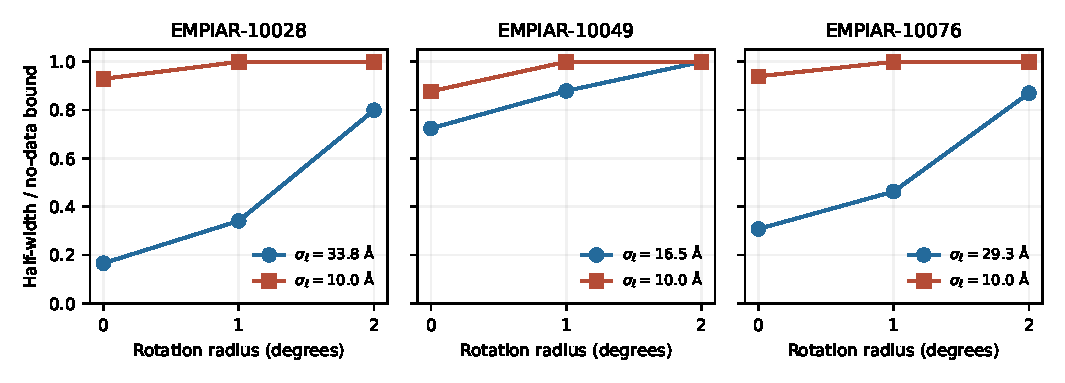
\includegraphics[width=.98\textwidth]{figures/revision-experimental.pdf}
\caption{Experimental sensitivity intervals with one inference particle per
exposure group. Kernel widths are Gaussian standard deviations, not FSC
resolutions. None of these intervals excludes zero. All 10\,\AA\ targets switch
to the no-data center and width at nonzero pose budgets. Supplied density/pose
classes and unverified common-noise/consensus-pose assumptions preclude an
experimental coverage claim.}
\label{fig:revisionexperimental}
\end{figure*}

All eighteen intervals contain their amplitude-aligned deposited-map value;
none excludes zero. This is a precision failure, not evidence of density
calibration. The 10\,\AA\ targets revert to no data at nonzero pose budgets.
The earlier 128-particle attempt on 10028 is also retained; it additionally
requires unverified independence within repeated exposure groups.

\subsection{Uniform CTF sensitivities}
For fixed voltage, spherical aberration and amplitude contrast $a$,
$C=\sin(\gamma-\arcsin a)$. If each defocus axis can change by $d$ and its
astigmatism angle by $b$ radians, a conservative defocus error is
$d+|\mathrm{df}_U-\mathrm{df}_V|\sin(\min(b,\pi/2))$. Multiplying by
$\pi\lambda s^2$ and adding the phase-shift radius bounds the phase error.
Evaluate the exact sine range on that interval, then multiply by the positive
relative gain/B-factor range. This yields an absolute transfer envelope
$e_{iq}$ without division by a CTF zero.

For any allowed pose, a complex Fourier wave has unit modulus on the unit-volume
cube. Therefore the additive CTF bias is bounded by
\begin{equation}
 b_{\rm CTF}\le (B+P)\sum_{iq}
       |w_{iq,\mathbb C}|e_{iq}/\sigma.
\end{equation}
This term can be combined with the nominal-CTF pose bound, including simultaneous
errors, but discards cancellations and is not optimized jointly with them.
Table~\ref{tab:revisionctf} applies it to all six saved radius-12 fixed-pose
fine-feature fits. Defocus uncertainty of 100\,\AA\ already causes two no-data
fallbacks; all six fall back at 500\,\AA\ and under the combined sensitivities.
These negative results diagnose a loose audit, not an impossibility theorem for
other estimators or a calibrated distribution of experimental CTF error.
\begin{table*}[t]
\centering\small
\begin{tabular}{lrr}
\toprule
CTF sensitivity & Relative half-width & No-data cases\\
\midrule
Nominal & 0.120--0.238 & 0/6\\
Defocus $\pm100$\,\AA & 0.647--1.000 & 2/6\\
Defocus $\pm500$\,\AA & 1.000--1.000 & 6/6\\
Combined nuisance bounds & 1.000--1.000 & 6/6\\
\bottomrule
\end{tabular}
\caption{Declared CTF-error envelopes added to all six fixed-pose radius-12 fine-feature fits. The combined setting is 100\,\AA\ defocus, $2^\circ$ astigmatism angle, $1^\circ$ phase, 5\% gain and 10\,\AA$^2$ relative B-factor. Radii are sensitivities, not calibrated errors. The triangle bound discards cancellation; its vacuity is not an impossibility result for other methods.}
\label{tab:revisionctf}
\end{table*}

